\documentclass[10pt,unicode]{beamer}
\usetheme{ttiposter}

% geometries

\geometry{paper=a4paper,landscape}

% packages

\usepackage{luatexja}
\usepackage{amsmath}
\usepackage{graphicx}
\usepackage[labelformat=empty]{caption}
\usepackage{subcaption}
\captionsetup{compatibility=false}
\usepackage{setspace}
\AtBeginDocument{% HACKING
  \addtolength\abovedisplayskip{-1.5\baselineskip}
  \addtolength\belowdisplayskip{-0.5\baselineskip}
}

% miscellaneous commands

%\definecolor{tenjugreen}{rgb}{0.4,0.8,0.4}
\newcommand{\columnsize}{0.32}
\newcommand{\tablefontsize}{\small}
\newcommand{\itemtitle}[1]{{\normalsize #1} \\}
\newcommand{\arrow}{{\color{ttiblue} →}\hspace{1ex}}
\newcommand{\notable}[1]{\textbf{\color{orange} #1}}
\newcommand{\keyword}[1]{\textbf{\color{red} #1}}

% title setting

\title{カテゴリ間の関連性を利用した多層ニューラルネットワークによる文書分類}
\author{外山洋太、三輪誠、佐々木裕}
\institute{豊田工業大学 工学部 先端工学基礎学科}
\date{}


\begin{document}
\begin{frame}{}
\maketitle
\begin{columns}[t]

\begin{column}{\columnsize\textwidth} % first
  \begin{block}{背景と目的}
    \begin{itemize}
      \item 文書を複数のカテゴリについて多値分類 \\
      (カテゴリ:ラベルが付けられる各項目のこと)
      \item 従来の手法[1]では...
        \begin{itemize}
        \item カテゴリ同士の関連性を\notable{手動で変化}させ考慮 \\
          \arrow \keyword{多層ニューラルネットワーク}による\notable{自動化}
        \item 文書の数値表現であるBoWは文書内の語順を無視 \\
          \arrow \keyword{パラグラフベクトル}の使用により表現をより正確に
        \end{itemize}
    \end{itemize}
  \end{block}

  \begin{figure}
    \begin{subfigure}{0.55\columnwidth}
      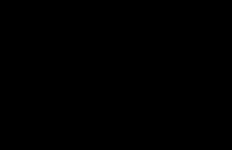
\includegraphics[width=\textwidth]{fig/reviewcomment.png}
    \end{subfigure}
    \begin{subfigure}{0.35\columnwidth}
      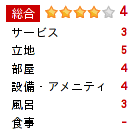
\includegraphics[width=\textwidth]{fig/reviewpoints.png}
    \end{subfigure}
    \caption{カテゴリ毎のラベルが付いたレビューの例}
  \end{figure}

%  \begin{block}{関連研究}
%    \begin{itemize}
%      \item 隠れ状態を用いたホテルレビューのレーティング予測 \\
%        文書内の各文に対して推定した隠れレーティングと
%        レビュー全体のレーティングとの繋がりを手動で変化させる \\
%        \arrow カテゴリ間の関連性を考慮
%      \item \keyword{vLBL+vLBL(c)}による\keyword{パラグラフベクトル}の生成 \\
%        \begin{itemize}
%          \item {\normalsize パラグラフベクトル} \\
%            \notable{語順を考慮}した文書の数値表現。
%            文書分類に有用であることが実験により示しされている。
%          \item {\normalsize vLBL+vLBL(c)} \\
%            \notable{単語同士の位置関係を考慮}した単語ベクトルの学習手法。
%            パラグラフベクトルまたは文ベクトルも同時に学習可能。
%        \end{itemize}
%    \end{itemize}
%  \end{block}

  \begin{block}{提案手法}
    \begin{itemize}
      \item vLBL+vLBL(c)の応用手法によって生成したパラグラフベクトル
        及び文ベクトル \\
        パラグラフベクトルに加え文ベクトルを導入したvLBL+vLBL(c)を提案し、
        \notable{語順と単語同士の位置関係を考慮}した文書の数値表現を生成
        \arrow 文書の意味を的確に表現
      \item 分類器としての多層ニューラルネットワーク
        \arrow カテゴリ間の関連性を自動的に考慮
    \end{itemize}
  \end{block}
\end{column} % first

\begin{column}{\columnsize\textwidth} % second
    \begin{figure}
      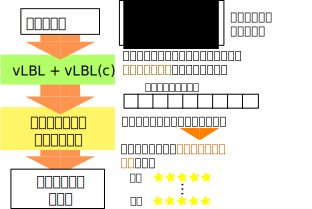
\includegraphics{fig/architecture.png}
      \caption{文書データからのカテゴリ毎のラベル推定}
    \end{figure}

    \begin{gather*}
      g = \sum_t \left\{ \log\sigma(s(t))
          + \sum^K_{t' \sim P_n} \log(1 - \sigma(s(t'))) \right\} \\
      s(t) = {\bf c}_t \cdot {\bf w}_t
             + {\bf c}^{loc}_t \cdot {\bf w}^{loc}_t + b_t \\
      \left(
      \begin{matrix}
        t : 現在の単語の位置 \\
        c_t, w_t : 文脈、単語を表すベクトル \\
        s : 位置関係を考慮した単語と文脈の類似度 \\
        σ : シグモイド関数
      \end{matrix}
      \right)
    \end{gather*}

    \begin{itemize}
      \item 現在の単語t \arrow 文脈との意味を近く
      \item 文脈外の単語t' \arrow 文脈との意味を遠く
    \end{itemize}

    \begin{figure}
      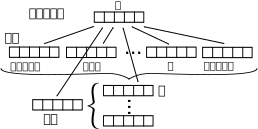
\includegraphics{fig/vectors.png}
      \caption{単語及び文、文章ベクトルの学習}
    \end{figure}
\end{column} % second

\begin{column}{\columnsize\textwidth} % third
  \begin{block}{予備実験}
    vLBL+vLBL(c)とSVMまたは多層NNを用い、
    従来の手法[1]と同じ多値分類問題の精度を測定

    \begin{itemize}
      \item \itemtitle{目的}
      \begin{itemize}
        \item パラグラフベクトルの有効性の調査
        \item 従来手法との比較による目標設定
      \end{itemize}

      \item \itemtitle{実験設定}
      \begin{itemize}
        \item 入力データは、各レビューのコメント部分と7カテゴリのレーティングの
        組(各カテゴリのレーティングは評価なしを含む6段階評価)
        \item 訓練データ:300,000件、評価データ:10,000件
        \item 多層NNの入力は位置を考慮した及び考慮していない
        2つのパラグラフベクトル
      \end{itemize}

      \item \itemtitle{結果及び考察}
      \begin{itemize}
        \item 多層NNを用いた場合でも、従来の手法[1]における精度を10pp以上
          下回っている \\
          \arrow 表現力の高い文書の数値表現を評価や、
          多層NNのパラメータ最適化が必要
      \end{itemize}
    \end{itemize}

    \begin{table}
    \tablefontsize
    \caption{点数推定プログラムのパラメータ設定}
    \label{table:parameters}
    \begin{tabular}{l | r}
    項目 & 値 \\
    \hline
    学習する単語の範囲 & 前後5単語 \\
    単語の最少出現回数 & 5回 \\
    ベクトルの次元数 & 400 \\
    中間層の数 & 1 \\
    入力層でのニューロン数 & 800個 \\
    中間層でのニューロン数 & 200個
    \end{tabular}
    \end{table}

    \begin{table}
    \tablefontsize
    \caption{各手法における点数推定精度}
    \begin{tabular}{l | r}
    項目 & 点数推定の精度(\%) \\
    \hline
    実験での手法(SVM)& 33.6 \\
    実験での手法(多層NN)& 37.7 \\
    従来の手法[1] & 48.3
    \end{tabular}
    \end{table}
  \end{block} % 実験

  \begin{block}{今後の課題と改善策}
    \begin{itemize}
      \item 文ベクトルの評価
      \item 多層NNのパラメータ最適化
      \item 提案手法の有用性の評価
    \end{itemize}
  \end{block} % まとめ

  参考文献 \\
  \begin{itemize}
  \item 藤谷宣典ら, 隠れ状態を用いたホテルレビューのレーティング予測.
  言語処理学会 第21回年次大会, 2015. \\
  \item Quoc Le et al., Distributed Representations of Sentences and Documents.
  ICML 2014, 2014. \\
  \item 森洸樹ら, 英文穴埋め問題における文章ベクトルと学習データの質の影響.
  第222回自然言語処理研究会, 2015.
  \end{itemize}
\end{column} % third

\end{columns}
\end{frame}
\end{document}
